\section{Разработка аппаратно-программного комплекса}

Для разработки программно-аппаратного комплекса, необходимо определиться, какую платформу использовать для реализации.

Для реализации поставленной задачи был выбран одноплатный компьютер Raspberry Pi 3 model B с 40 контактами GPIO, адресная светодиодная лента, состоящая из 60 светодиодов WS2812b.

\subsection{Разработка аппаратной части комплекса}

Для управления светодиодной лентой, необходима генерация ШИМ-сигнала, подаваемая на контакт Din светодиодной ленты. Это, в свою очередь накладывает свои требования к генератору ШИМ-сигнала.

Для передачи информации, на контакт Din светодиодной ленты должны поступать последовательности по 24 бита, или по 3 байта, которые отвечают за цвет определённого светодиода. При модуляции используются длительности импульсов, согласно таблице~\ref{tab:ws2812__data_transfer_time}~\cite{Worldseim}.

\begin{table}[H]
  \caption{Длительность импульсов для управления светодиодом WS2812b}
  \label{tab:ws2812__data_transfer_time}
  \begin{tabular}{|c|l|c|}
  \hline
  \textbf{Обозначение} & \multicolumn{1}{c|}{\textbf{Описание}} & \textbf{Время} \\ \hline
  T0H                  & код "0", время высокого уровня         & 0,35 мкс       \\ \hline
  T1H                  & код "1", время высокого уровня         & 0,9 мкс        \\ \hline
  T0L                  & код "0", время низкого уровня          & 0,9 мкс        \\ \hline
  T1L                  & код "1", время низкого уровня          & 0,35 мкс       \\ \hline
  RES                  & время низкого уровня                   & 50 мкс         \\ \hline
  \end{tabular}
\end{table}

Визуально ШИМ импульсы представлены на рисунке~\ref{img:WS2812__PWM_codes}.

\begin{figure}[H]
  \centering
  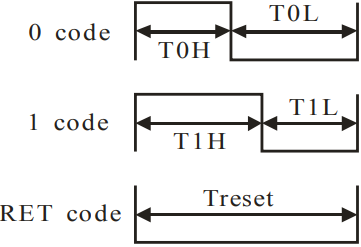
\includegraphics[height=0.2\textheight]{assets/images/practical/PWM__codes.png}
  \caption{ШИМ импульсы для управления WS2812b}
  \label{img:WS2812__PWM_codes}
\end{figure}

При кодировании цвета светодиода, последовательность из 24 бит представляется как 3 подряд идущих пакета, описывающих определённый основной сигнал. Первый пакет описывает зелёную составляющую цвета, второй --- красную, третий --- синюю. Биты в пакетах идут от старшего к младшему.

Например, для описания цвета, представленного в RGB как (18, 88, 160), необходимо преобразовать его в GRB, (88, 18, 160). Затем перевести их в двоичный вид, 01011000 00010010 10100000, и подать на вход Din светодиодной ленты в ШИМ. Для данного примера, ШИМ будет выглядеть как на рисунке~\ref{img:WS2812__PWM_example}.

\begin{figure}[H]
  \centering
  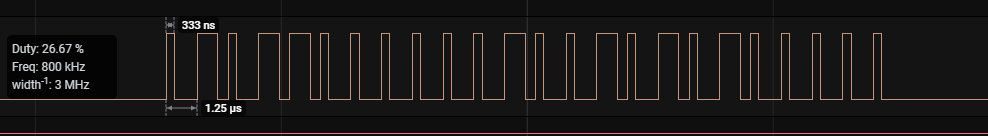
\includegraphics[width=0.9\textwidth]{assets/images/practical/PWM__example.jpg}
  \caption{Пример ШИМ для кодирования цвета}
  \label{img:WS2812__PWM_example}
\end{figure}

Для генерации ШИМ можно использовать расположенные на плате Raspberry Pi GPIO контакты.

Для программной генерации ШИМ можно использовать все контакты GPIO, но при таком подходе часть аппаратных ресурсов платформы будет тратиться на генерацию и кодирование импульсов, что влечёт за собой уменьшение производительности всей системы. Для аппаратной генерации ШИМ предназначены контакты GPIO12, GPIO13, GPIO18, GPIO19 Raspberry Pi. В этом случае достигается большая производительность системы и упрощение для разработчика при работе с напряжением на контактах GPIO. Полная карта контактов Raspberry Pi представлена на рисунке~\ref{img:raspberrypi__GPIO_pinout_diagram}.

\begin{figure}[H]
  \centering
  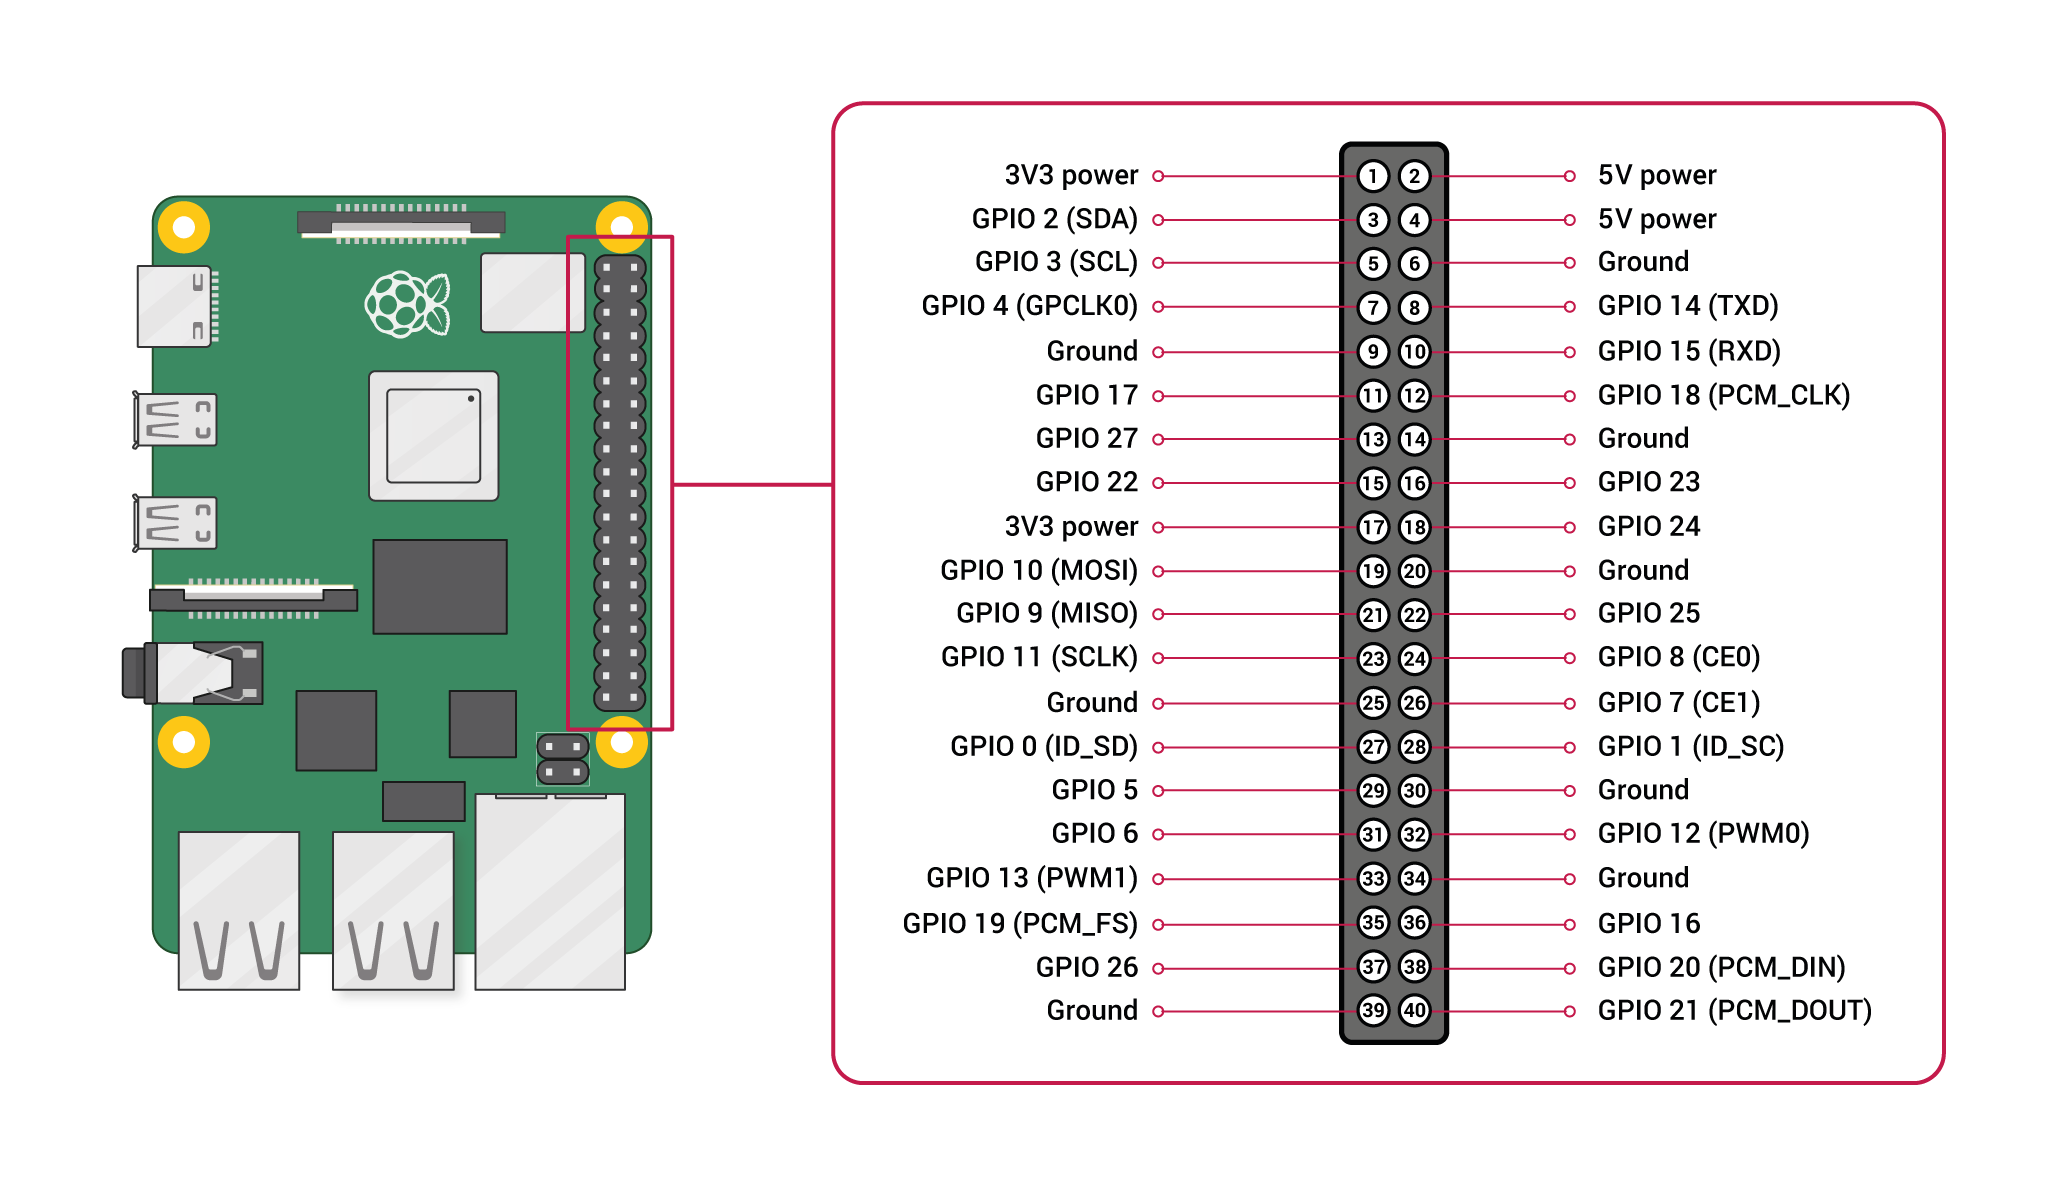
\includegraphics[width=0.9\textwidth]{assets/images/practical/GPIO-Pinout-Diagram.png}
  \caption{Карта GPIO контактов Raspberry Pi}
  \label{img:raspberrypi__GPIO_pinout_diagram}
\end{figure}

Ввиду описанных выше факторов, для генерации ШИМ был выбран контакт GPIO18, обозначен номером 12 на карте~\ref{img:raspberrypi__GPIO_pinout_diagram}. Также, согласно карте GPIO контактов, в качестве контакта заземления был выбран контакт 6.

В следствие этого, был разработан итоговый макет программно-аппаратного комплекса. Макет представлен на рисунке~\ref{img:all__schema}.

\begin{figure}[H]
  \centering
  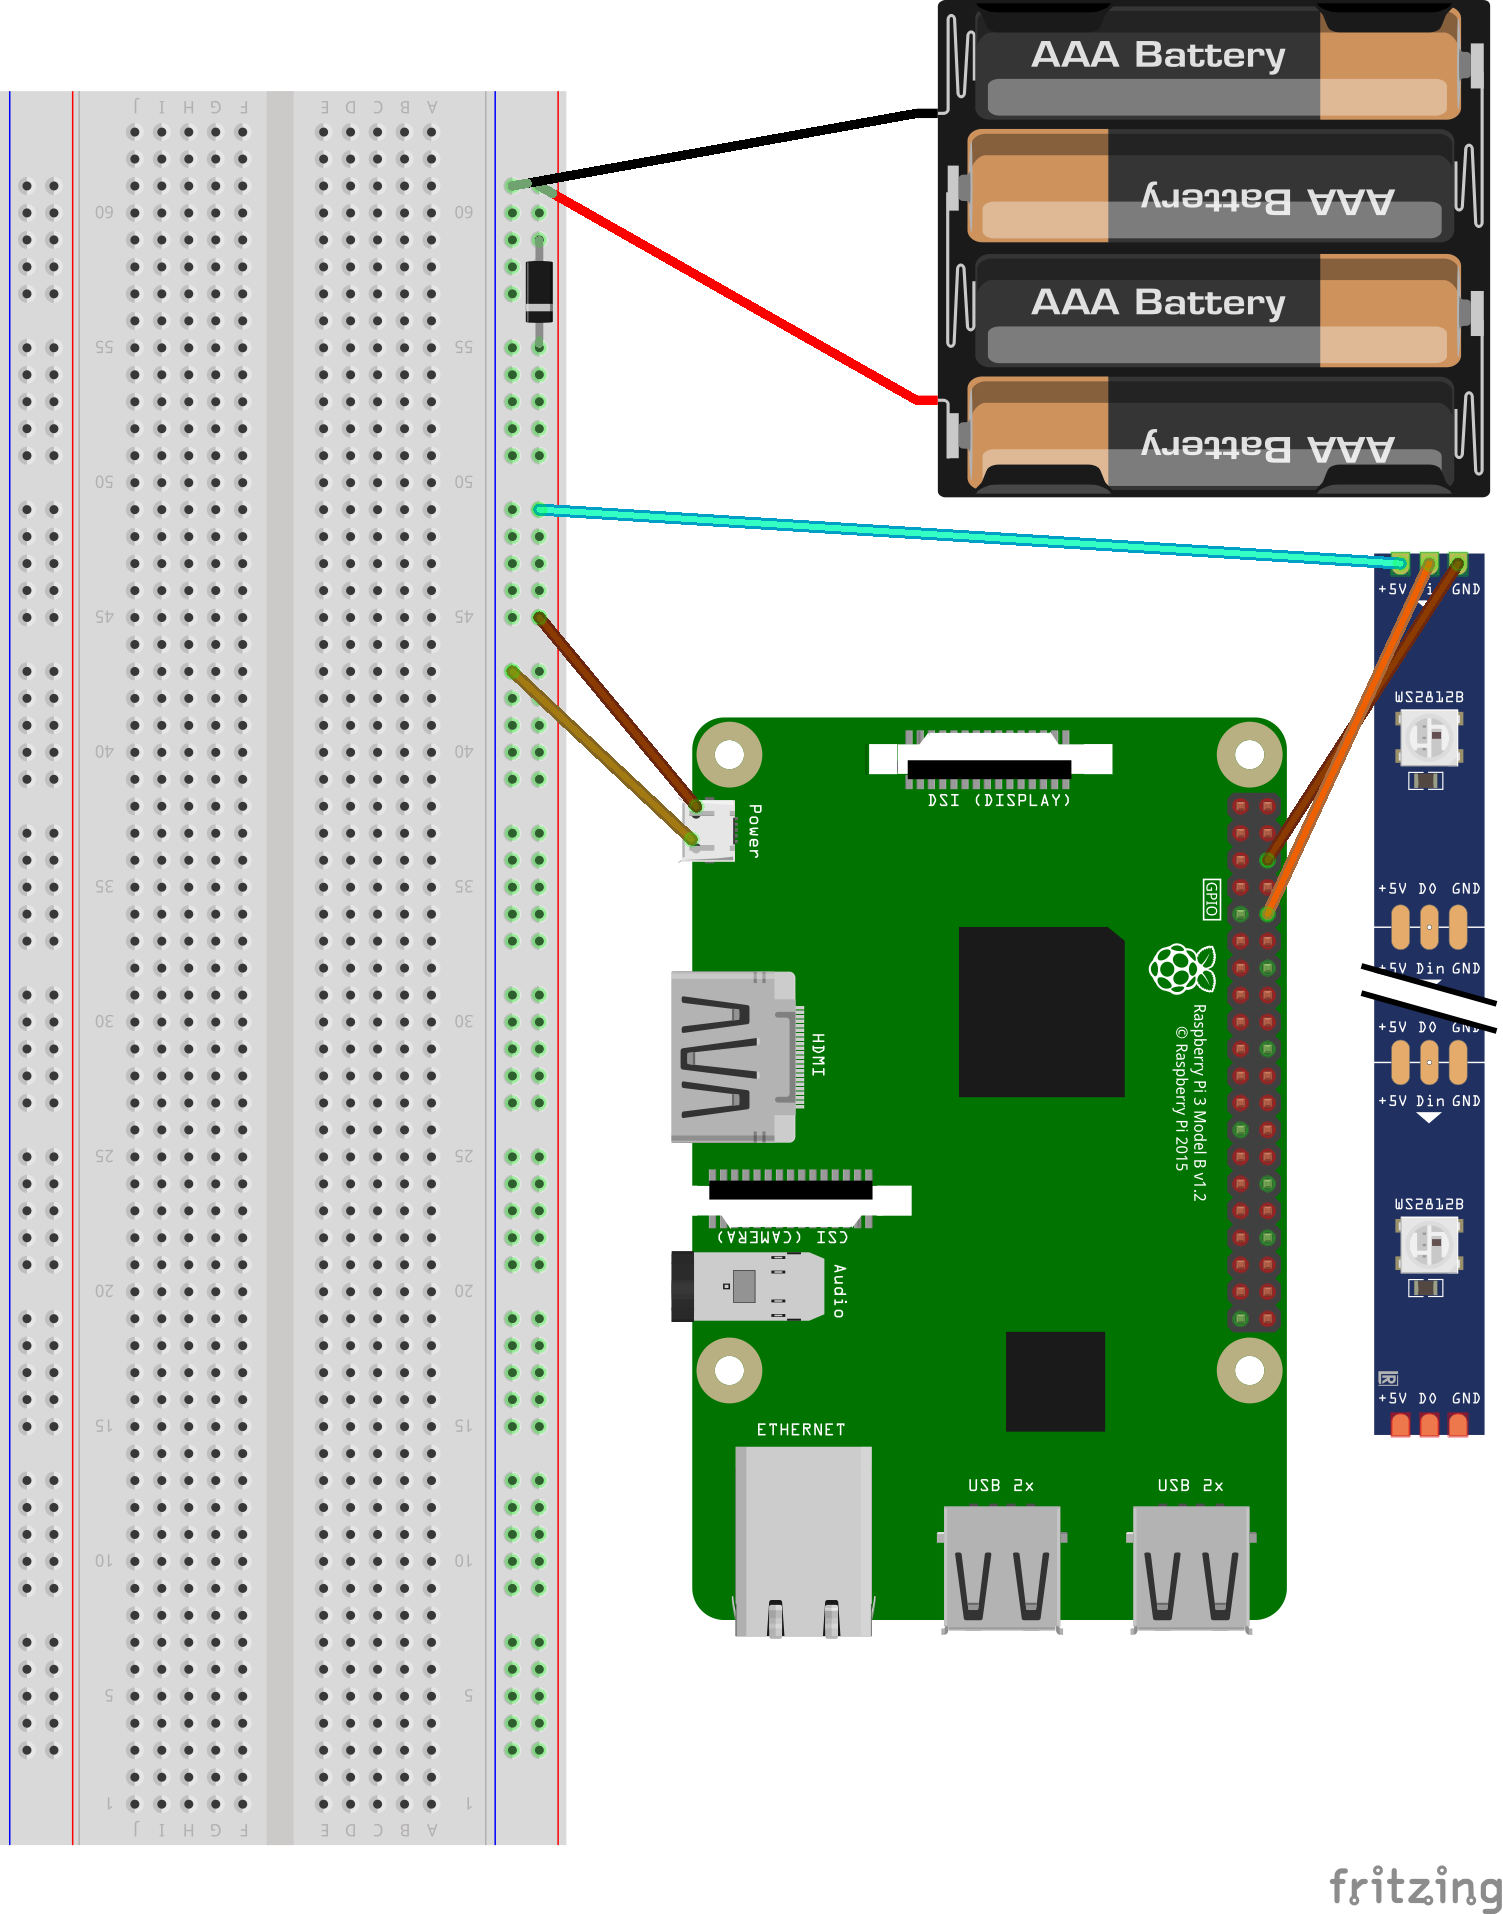
\includegraphics[angle=-90, width=0.9\textwidth]{assets/images/practical/Итоговая архитектура программно-аппаратного комплекса.png}
  \caption{Итоговый макет программно-аппаратного комплекса}
  \label{img:all__schema}
\end{figure}

Согласно макету~\ref{img:all__schema} была собрана и протестирована работоспособность системы. На этом разработку аппаратной части комплекса можно считать завершённой. Собранный комплекс представлен на рисунке~\ref{img:all__hard}.

\begin{figure}[H]
  \centering
  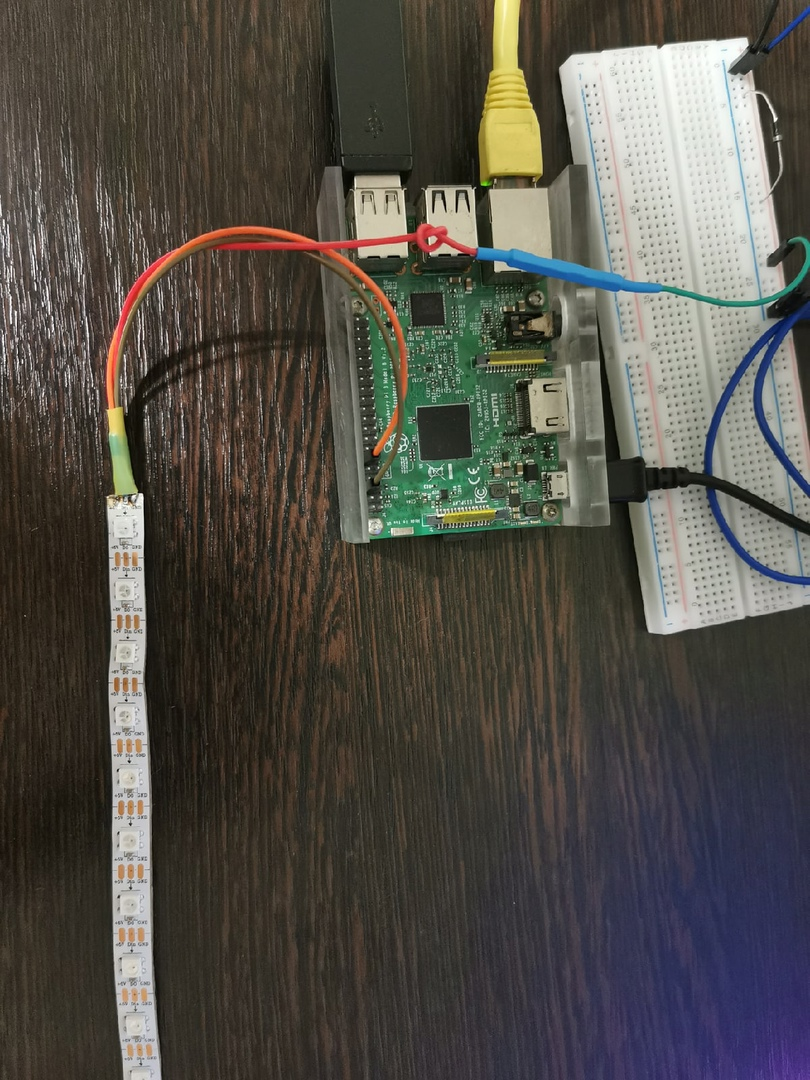
\includegraphics[angle=90, width=0.9\textwidth]{assets/images/practical/Полная схема.jpg}
  \caption{Собранный комплекс}
  \label{img:all__hard}
\end{figure}



\subsection{Разработка программной части комплекса}

\subsubsection{Операционная система Manjaro}
В качестве операционной системы для управления Raspberry Pi был выбран дистрибутив Manjaro.

Manjaro является дистрибутивом Linux, основанным на Arch Linux, который позиционируется как открытая и лёгкая операционная система. Также Arch Linux и Manjaro обладают подробной документацией.

В Manjaro по-умолчанию используется ALSA в качестве звуковой подсистемы, поэтому для записи звуковых потоков используется утилита arecord, а для воспроизведения --- aplay.

Manjaro использует пакетный менеджер pacman, упрощающий управление пакетами. Для поддержания пакетов в актуальном состоянии, pacman синхронизируется с базами данных пакетов Manjaro посредством зеркал. Также возможна и установка пакетов ``вручную'' из исходных кодов.

Для начала разработки, необходимо установить все необходимые пакеты, такие как gcc, предоставляющую компиляторы языков C и C++, make, предоставляющую сборку утилит из исходных кодов, sudo, упрощающую выполнение команд от имени администратора, и других пакетов. Для установки этой группы пакетов, необходимо выполнить следующую bash-команду:

\begin{lstlisting}[style=ES6, language=bash]
  sudo pacman -Syy base-devel
\end{lstlisting}

При установке пакетов произойдёт полная синхронизация баз данных пакетов, так как был указан параметр ``yy''.

\subsubsection{Node.JS}

В качестве основного языка разработки комплекса был выбран язык JavaScript (JS). Для взаимодействия с операционной системой используется среда выполнения JS --- NodeJS (Node). Чтобы иметь возможность выполнять Node-скрипты, необходимо предварительно установить пакет `nodejs' с помощью менеджера пакетов pacman, либо с помощью менеджера версий nvm. Ввиду своей простоты, была произведена установка с помощью pacman.

\begin{lstlisting}[style=ES6, language=bash]
  sudo pacman -S nodejs
\end{lstlisting}

Вместе с установкой Node, производится установка Node Package Manager (npm), с помощью которого можно управлять Node-проектами и устанавливать Node-пакеты.

Для создания нового проекта используется npm. Для инициализации проекта, необходимо выполнить команду `npm init -y', которая создаст в текущей директории файл package.json, в котором хранится вся информация о проекте: название, автор, текущая версия, команды управления, используемые пакеты, или зависимости, и другая информация.

\subsubsection{Пакеты для управления алресными светодиодными лентами}

Для управления адресными светодиодными лентами с помощью Node, наибольшей популярностью обладают 3 пакета~\cite{npm}:

\begin{itemize}
  \item node-pixel;
  \item rpi-ws281x;
  \item rpi-ws281x-native.
\end{itemize}

Node-pixel является наиболее популярным пакетом, но он также является самым ``тяжёлым'' пакетом и предполагает использование какой-либо другой платы, например, Arduino Nano, с помощью которой происходит управление светодиодной лентой. В этом случае Raspberry Pi выполняет роль интерпретатора языка Node, а плата, принимая полученные по I2C-шине данные, управляет светодиодной лентой. Данный пакет не был использован в проекте, так как его возможности излишни.

Rpi-ws281x и rpi-ws281x-native являются пакетами, близкими по популярности. Они предоставляют возможность прямого управления светодиодной лентой с RPI, без использования каких-либо промежуточных контроллеров.

При разработке программной составляющей проекта был использован пакет rpi-ws281x-native, ввиду более подробной документации и использования при выполнении нативных привязок GPIO.

\subsubsection{Создание дочерних процессов}

Запуск системных утилит с помощью Node можно произвести с помощью запуска дочерних процессов.

Node обладает встроенным модулем `child\_process', предоставляющий возможность запуска, завершения и управления дочерними процессами. Существует 4 способа запуска дочерних процесса~\cite{node}:

\begin{itemize}
  \item child\_process.exec() --- exec;
  \item child\_process.execFile() --- execFile;
  \item child\_process.fork() --- fork;
  \item child\_process.spawn() --- spawn.
\end{itemize}

Exec и execFile используются, когда необходим запуск команды или файла, содержащего команды, или исполняемого файла, без возможности управления его стандартными потоками. В этом случае создаётся отдельный процесс, выполняемый, пока на одном из стандартных потоков не появятся данные. Например, эти команды можно использовать для запуска какой-либо системной службы или получения информации о файле.

Spawn используется для запуска команды с некоторыми параметрами запуска. В этом случае возможно управление стандартными потоками ввода, вывода и ошибок. Также, процесс, запущенный с помощью spawn будет активен, пока не получит терминальный сигнал от родительского процесса или от операционной системы.

Fork является подвидом spawn, предоставляющим возможность запуска нового Node процесса.

Для запуска процессов, выполняющих команды aplay и arecord, был использован способ spawn.

Например, используя скрипт, представленный в листинге~\ref{lst:node__spawn_pipe}, можно запустить процессы, выполняющие запись и воспроизведение звука, перенаправив выходной стандартный поток процесса записи во входной стандартный поток процесса воспроизведения.

\begin{lstlisting}[style=ES6, caption={Пример запуска процессов и перенаправления потоков процессов}, label={lst:node__spawn_pipe}]
const arecordProcess = spawn('arecord', [
    '-t', 'raw'
]);

const aplayProcess = spawn('aplay', ['-',
  '-t', 'raw'
]);

arecordProcess.stdout.pipe(aplayProcess.stdin);
\end{lstlisting}

\subsubsection{Управление адресной светодиодной лентой}

Для управления адресной светодиодной лентой используется пакет rpi-ws281x-native, который предоставляет нативные привязки GPIO для более эффективного управления светодиодными лентами.

При инициализации объекта управления светодиодной лентой, необходимо указать следующие параметры:

\begin{itemize}
  \item count --- количество светодиодов в ленте;
  \item gpio --- выход GPIO, к которому подключена лента. По-умолчанию управление происходит с помощью GPIO18;
  \item invert --- изменение выходного сигнала. Применяется, если используется логический преобразователь уровней. По-умолчанию значение false;
  \item brightness --- яркость, применяемая ко всем светодиодам в ленте. По-умолчанию максимальна, 255;
  \item stripType --- тип светодиодов в ленте. По-умолчанию WS2812.
\end{itemize}

Данные о ленте хранятся в виде массива чисел, где каждому элементу массива соответствует определённый светодиод. Обращение к светодиодам происходит по индексам.

Для отправления необходимого состояния на светодиодную ленту, используется метод render().

Перед тем, как завершить работу с лентой, необходимо очистить данные, хранящиеся на контроллерах её светодиодов. Это можно сделать с помощью метода reset(), который очистит данные на контроллерах светодиодов, и finalize(), который отключает драйвер управления светодиодной лентой и высвобождает ресурсы.

Например, в листинге~\ref{lst:node__rainbow} представлен скрипт, который запускает анимацию переливания цветов для всей светодиодной ленты.

\lstinputlisting[style=ES6, caption={Пример скрипта, запускающего анимацию переливания цветов на светодиодной ленте}, label={lst:node__rainbow}, linerange={19-29, 33-48}, consecutivenumbers=true]{assets/listings/practical/rainbow.js}

Пример работы эффекта переливания представлен на рисунке~\ref{img:ws2812__rainbow}.

\begin{figure}[H]
  \centering
  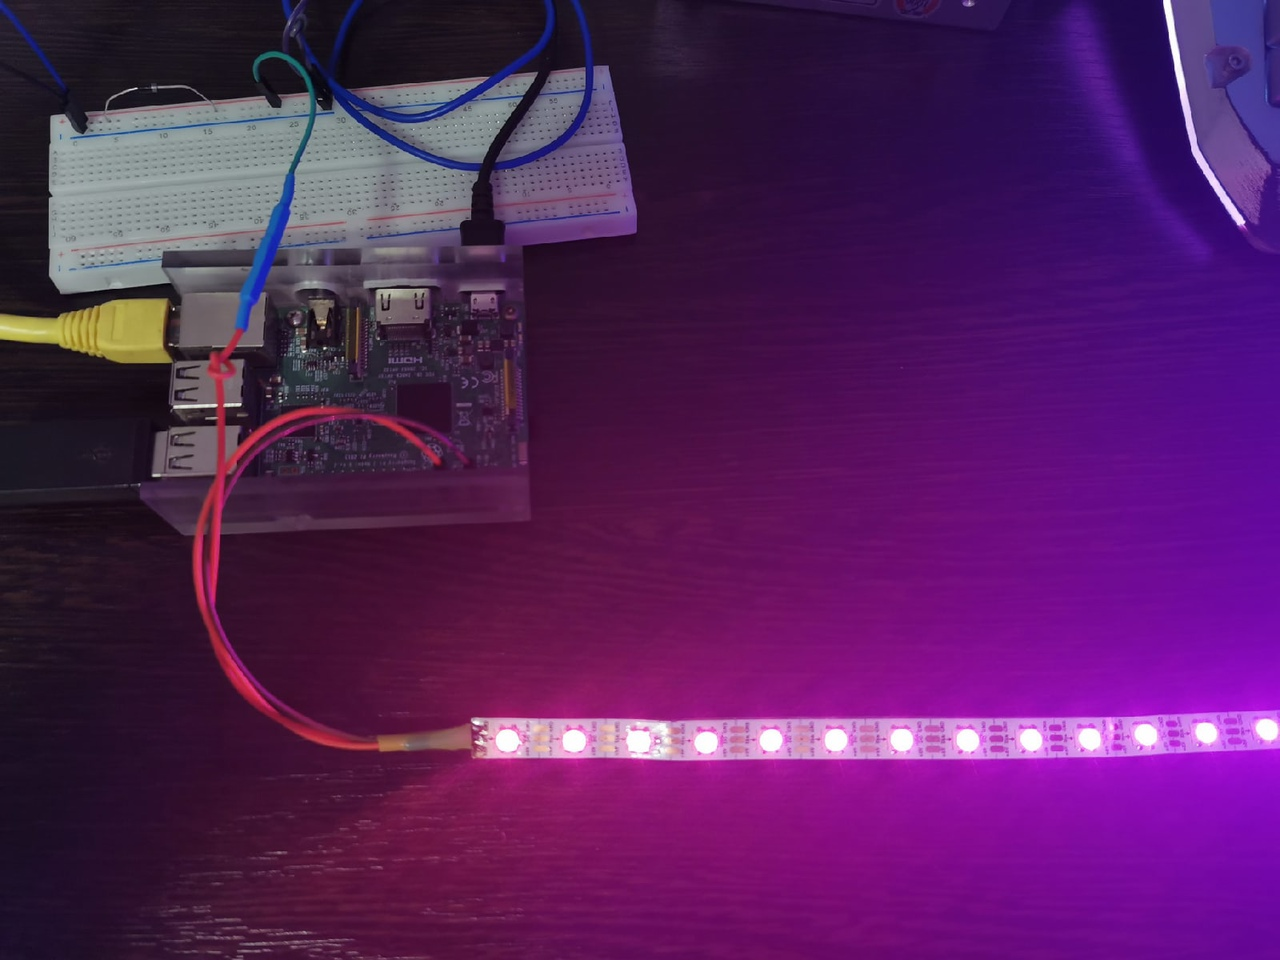
\includegraphics[width=0.9\textwidth]{assets/images/practical/Эффект переливания.jpg}
  \caption{Эффект переливания}
  \label{img:ws2812__rainbow}
\end{figure}

В случае, если необходимо, чтобы цвета выходили из центра светодиодной ленты и расходились в стороны, тогда скрипт будет выглядеть, как показано в листинге~\ref{lst:node__shift}. Предполагается, что число светодиодов в ленте чётное.

\lstinputlisting[style=ES6, caption={Пример функции, запускающего анимацию выхода цвета из центра светодиодной ленты в стороны}, label={lst:node__shift}, linerange={23-39}, consecutivenumbers=true]{assets/listings/practical/LED.js}

Пример работы эффекта выхода цветов из середины ленты представлен на рисунке~\ref{img:ws2812__shift}.

\begin{figure}[H]
  \centering
  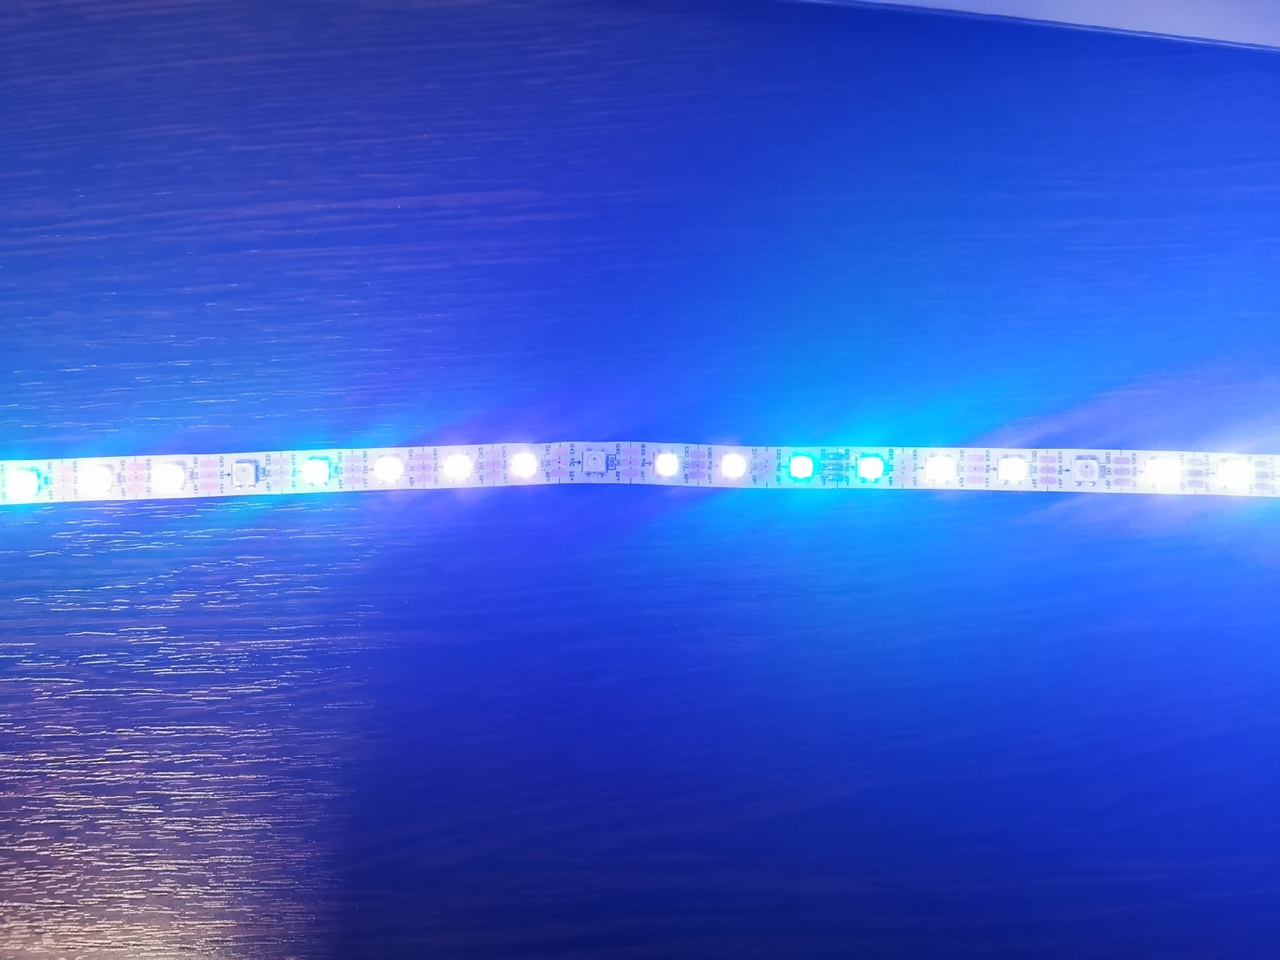
\includegraphics[width=0.9\textwidth]{assets/images/practical/Эффект из центра.jpg}
  \caption{Эффект выхода цветов из середины ленты}
  \label{img:ws2812__shift}
\end{figure}

В этой функции на вход поступают массив, описывающий светодиоды в ленте, и новый цвет, который необходимо отобразить начиная с центра. Сначала находится индекс центрального элемента, затем смещаются на один влево/вправо цвета светодиодов, и добавляется новый цвет. Возвращаемым значением является новое состояние светодиодной ленты.

Для отображения полученного состояния на светодиодной ленте, можно воспользоваться функцией, предложенной в листинге~\ref{lst:node__render}.

\lstinputlisting[style=ES6, caption={Пример функции отображения нового состояния светодиодной ленты}, label={lst:node__render}, linerange={84-89}, consecutivenumbers=true]{assets/listings/practical/LED.js}

Полный код управления светодиодной лентой представлен в приложении~\ref{lst:node__all_LED}.

\subsubsection{Обработка звука}

Дочерний процесс, в котором выполняется команда arecord, в случае работы в одноканальном режиме с частотой дискретизации 8000 Гц и битовой глубиной 8 бит, возвращает в стандартный поток вывода каждую секунду 8000 записей со значениями от 0 до 255, показывающими уровень шума в соответствующий момент времени.

Для преобразования полученного звукового потока в световой, необходимо разработать и реализовать процесс обработки звука.

Был выбран следующий способ обработки:

\begin{itemize}
  \item Каждый интервал времени t1 получаются значения, полученные после импульсно-кодовой модуляции звука, и выбирается максимальный элемент max1, а именно его значений и его индекс;
  \item Проверяется, является ли полученное значение максимального элемента max1 большим чем некоторый порог. Если значение ниже этого порога, то значение максимального элемента max1 становится равным 0;
  \item Сравнивается значение полученного максимального элемента max1 и текущим максимальным значением max. Если первое больше, то максимальный элемент max становится равным max1;
  \item Параллельно этому процессу, каждый интервал времени t2 получается значение максимального элемента max, это значение переводится в цветовое представление, и значение максимального элемента становится равным -1.
\end{itemize}

Фрагмент функции обработки звукового потока представлен в листинге~\ref{lst:node__signalProcessing}.

\lstinputlisting[style=ES6, caption={Фрагмент функции обработки звукового потока}, label={lst:node__signalProcessing}, linerange={48-68}, consecutivenumbers=true]{assets/listings/practical/index.js}

Полный код реализации поставленной задачи представлен в приложении~\ref{lst:node__all_index}.


% 
%\input{modules/practical/}
